\section{Experimental setup}
\label{sec:exp_setup}

In this section, we describe our experimental setup based on ns-2 used to compare TE schemes with respect to their impact on application performance. 
We chose ns-2 as it is well-suited for simulating thousands of flows in an ISP network at the packet level while also incorporating transport and application behavior in a fine-grained manner.

% Evaluating application performance accurately necessitates modeling application and transport behavior, especially their response to network characteristics, in a fine-grained manner. We chose ns-2 as the simulation platform as it is well-suited to simulate thousands of flows in an ISP network at the packet level while also incorporating transport and application behavior in a fine-grained manner.


%Below, we discuss (1) why this simulation infrastructure is necessary, (2)  how we simulate real traffic matrices using ns-2, and (3) the traffic engineering schemes, real ISP topologies, and real traffic matrices in our experiments.

%In this section we describe our ns-2 simulation infrastructure to compare application performance for traffic engineering methods. First we discuss why this simulation infrastructure is necessary,  next we explain how we simulate traffic matrices using ns-2, and then we describe the TE schemes we compare and the ISP topologies and traffic matrices in our simulation.

%Our goal is to study the impact of TE schemes on end-to-end application performance. TE impacts application performance in several ways. First, TE determines the utilization on backbone links in the network, which in turn influences the loss rate and queuing delay of those links. Second,  TE determines the route between PoPs in the network and thereby impacts path delays. These factors---propagation delay, queuing delay, and loss rate---primarily influence user-perceived application performance, e.g., the loss rate and path delay determines TCP performance as well as the quality of streaming applications.

% Evaluating application performance accurately necessitates modeling application and transport behavior, especially their response to network characteristics, in a fine-grained manner. We chose ns-2 as the simulation platform as it is well-suited to simulate thousands of flows in an ISP network at the packet level while also incorporating fine-transport and application behavior in a fine-grained manner.


%\label{fig:ISP_data}
%\begin{wrapfigure}[12]{r}{0.25\textwidth}\footnotesize
%  \begin{center}
%  \begin{tabular}{ p{0.7cm} | p{0.7cm} | p{0.8cm}  }
%\textbf{BW (Mbps)} &\textbf{US users \%}  & \textbf{Europe users \% } \\ \hline 
%0.25 & 4.9 &   1.5 \\
%2.0  & 38.1 & 26.2  \\
%5.0 & 32.4 & 57.8	\\
%10.0 & 20.0 & 14.5 \\
%20.0 & 4.6 & - \\
%  \end{tabular}
%  \end{center}
%  \caption{Bandwidth Distribution}
%\end{wrapfigure}
%\label{fig:bandwidth_distribution}

%in order to determine link utilization levels and evaluate cost functions based on them. But, these cost functions do not capture network wide application performance.  They can be biased by traffic on one or a few links and  do not take into account the path delay which is important for application performance.  Simulation is the simplest approach to get a reasonable estimate of application performance. Another approach we considered was using theoretical model e.g. fixed point \cite{fixedpoint} models for large number of network flows. Since these are theoretical models, they do contain modeling errors. Another reason, we excluded theoretical models is these models are  not well understood  for a network with multiple bottleneck links \cite{fixedpoint}. Since we use a simulation infrastructure, our experiments are prone to simulation errors. An even more accurate experiment would involve emulation ( e.g Emulab) or a  virtualized infrastructure (e.g. VINI \cite{VINI} ) but we restricted ourselves to doing ns-2 simulations because its ease of use enabled us to run large number of experiments.



\subsection{Simulating traffic matrices in ns-2}
\label{sec:sim_TM}

Figure~\ref{fig:simulation1} illustrates the experimental process. Each simulation has three inputs: (1) \textsl{ISP Topology} (2) a sequence of \textsl{File Arrivals} at each node based on the current \textsl{TM} (3) \textsl{Routing}, as computed using a \textsl{TE} scheme. %The slanted text refers to the corresponding block in Figure~\ref{fig:simulation1}.

We construct an ISP network topology from our dataset consisting of PoP-level ISP topology maps. PoPs are represented as nodes and links between these nodes are the backbone links of the ISP. Each PoP node has a number of users connected to it via separate access links. Each PoP node also has five server nodes connected to it via high capacity links that serve files to users. The number of user nodes in our simulation ranges from 300-6000 nodes and the capacity of backbone links varies from 50Mbps to 1Gbps.

\begin{figure}
 \begin{center}
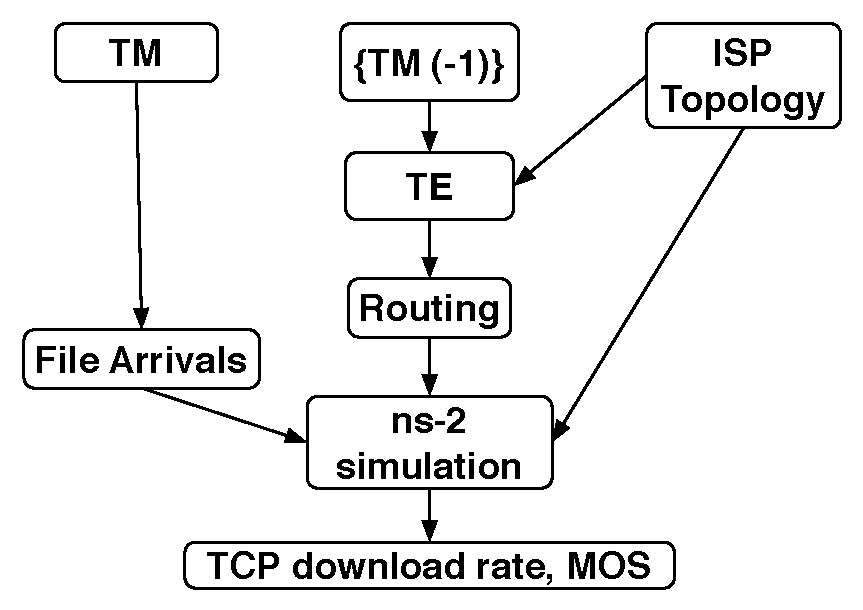
\includegraphics[scale=0.4]{final_images/Simulation1.pdf}
\caption{Block diagram of experiment process}
 \end{center}
 \label{fig:simulation1}
 \end{figure}
 
%\begin{figure}[tbh]
%  \begin{center}
%\includegraphics[scale=0.42]{}
% \end{center}
%\vspace{-0.1in}
%	  \caption{}
%  \label{fig:simulation1}
%\end{figure}

%\begin{figure}[tbh]
%  \begin{center}
%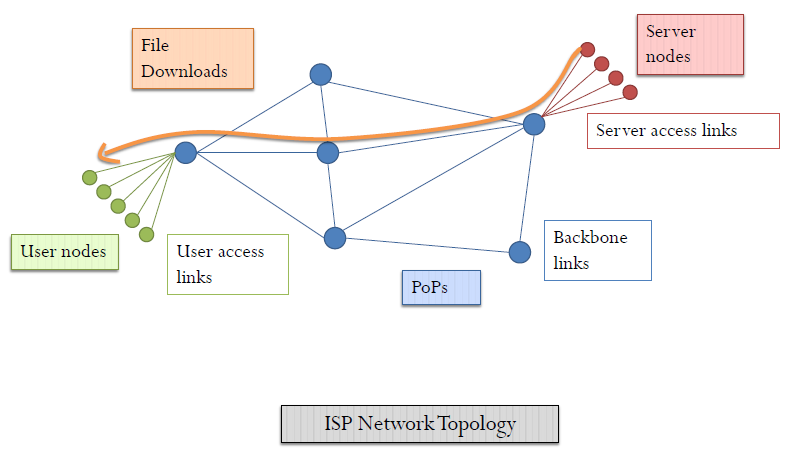
\includegraphics[scale=0.37]{final_images/expSetup.png}
% \end{center}
%\vspace{-0.1in}
%	  \caption{Diagram of an ISP network toplogy used in simulation}
%  \label{fig:isp_topology}
%\end{figure}


We translate a \textsl{TM} to a sequence of \textsl{File Arrivals} as follows. Suppose the traffic matrix entry from A to B is 100 Mbps and the duration being simulated is 200 seconds. During the experiment interval, we generate a sequences of file arrivals from A to B whose total size is 100Mbps $\times$ 200 seconds and the sizes are chosen from a realistic distribution.

A traffic engineering scheme \textsl{TE} calculates routing for \textsl{TM} based on a set of matrices \textsl{TM(-1)} which consists of either the current traffic matrix (for \opt) or a set of matrices from the previous traffic engineering {\em epoch} (for other TE schemes). The length of the epoch depends on {\em TE}, e.g., the epoch length for \optwt\  is 3 hours and for \cope\ is 1 day. When \textsl{TE}  yields a routing that splits flows across multiple paths between two nodes, the number of files assigned to each path is proportional to the flow along that path. We use  the source routing option in ns-2 to pin a file to a path. We note that the link utilization values obtained using this ns-2 methodology are consistent with those obtained using a simple linear program with the difference being at most 0.1.

%We are able to simulate matrices accurately using this method and the difference between empirical link utilization from ns-2 and the value obtained using a linear program based calculation is at most 0.1.

%We specify the path for each file using the source routing option in ns-2.


%\begin{table}[tb]\footnotesize
%    \subfigure[ISP Data]{\label{fig:ISP_data}
%  \begin{tabular}{ p{0.9cm} |  p{0.7cm} |  p{0.7cm} |   p{0.8cm} }
%\textbf{ISP} &\textbf{Nodes}  & \textbf{Links}  & \textbf{Duration of TM } \\ \hline
%US-ISP & 25 & 88 & 1hr\\ 
%Geant  & 22 & 68 & 15min \\
%Abilene & 12 & 30 & 5min	\\
%  \end{tabular}}
%    \subfigure[Bandwdith Distribution of Internet Users]{\label{fig:bandwidth_distribution}
%  \begin{tabular}{ p{0.7cm} | p{0.7cm} | p{0.8cm}  }
%\textbf{BW (Mbps)} &\textbf{US users \%}  & \textbf{Europe users \% } \\ \hline 
%0.25 & 4.9 &   1.5 \\
%2.0  & 38.1 & 26.2  \\
%5.0 & 32.4 & 57.8	\\
%10.0 & 20.0 & 14.5 \\
%20.0 & 4.6 & - \\
%  \end{tabular}}
%\caption{Simulation Data}
%\end{table}



In order to make the simulation complexity tractable, we scale down the topology and matrices.
ISP backbone link capacities run into tens of Gbps. Simulating such a network at scale even for 100 seconds would require sending data on the order of terabytes (or equivalently, a million 100KB files). Experimentally, we find that simulating at a tenth of this scale, i.e., 100K files, is feasible given the computational and memory constraints of our machines. A typical scale in our simulation is 1/20, i.e., we simulate the backbone link with 1/20 the capacity and also scale down the traffic between each source-destination pair accordingly.


%The scale of experiment determines the number of concurrent flows on a link. 

%A larger scale simulation has more concurrent flows in the network and makes the aggregate behavior more bursty.

\subsubsection{ISP topologies and traffic matrices}  We use datasets from the following three ISPs for our experiments:

\begin{figure*}\footnotesize
\begin{minipage}[b]{0.55\textwidth}
    \begin{tabular}{ l | c | c |   c }
%  \begin{tabular}{ p{0.9cm} |  p{0.7cm} |  p{0.7cm} |   p{1cm} }
\textbf{ISP} &\textbf{Nodes}  & \textbf{Links}  & \textbf{TM Duration} \\ \hline
Abilene & 12 & 30 & 5min	\\
&&&\\
Geant  & 22 & 68 & 15min \\
&&&\\
US-ISP & - & - & 1hr\\ 
  \end{tabular}
 \caption{ISP Data}
\label{fig:ISP_data}
\end{minipage}
\begin{minipage}[b]{0.45\textwidth}
  \begin{tabular}{ p{1.2cm} | p{1.5cm} | p{1.5cm}  }
\textbf{BW (Mbps)} &\textbf{US users \%}  & \textbf{Europe users \% } \\ \hline 
0.25 & 4.9 &   1.5 \\
2.0  & 38.1 & 26.2  \\
5.0 & 32.4 & 57.8	\\
10.0 & 20.0 & 14.5 \\
20.0 & 4.6 & - \\
  \end{tabular}
  \caption{Bandwidth Distribution}
\label{fig:bandwidth_distribution}
\end{minipage}
\end{figure*}

%
%\begin{figure}\footnotesize
%  \begin{center}
%    \begin{tabular}{ l | c | c |   c }
%%  \begin{tabular}{ p{0.9cm} |  p{0.7cm} |  p{0.7cm} |   p{1cm} }
%\textbf{ISP} &\textbf{Nodes}  & \textbf{Links}  & \textbf{TM Duration} \\ \hline
%Abilene & 12 & 30 & 5min	\\
%Geant  & 22 & 68 & 15min \\
%US-ISP & - & - & 1hr\\ 
%  \end{tabular}
% \caption{ISP Data}
%\label{fig:ISP_data}
%  \end{center}
%\end{figure}
%
%
%
%\begin{figure}\footnotesize
%  \begin{center}
%  \begin{tabular}{ p{1.2cm} | p{1.2cm} | p{0.8cm}  }
%\textbf{BW (Mbps)} &\textbf{US users \%}  & \textbf{Europe users \% } \\ \hline 
%0.25 & 4.9 &   1.5 \\
%2.0  & 38.1 & 26.2  \\
%5.0 & 32.4 & 57.8	\\
%10.0 & 20.0 & 14.5 \\
%20.0 & 4.6 & - \\
%  \end{tabular}
%  \end{center}
%  \caption{Bandwidth Distribution}
%\label{fig:bandwidth_distribution}
%\end{figure}
%


(1) \textbf{Abilene}, from the publicly available Abilene ISP data \cite{abilene}.
(2) \textbf{Geant}, the un-anonymized version of the Geant topology obtained from the TotemData \cite{TotemData} project personnel. 
(3) \textbf{US-ISP}, a large Tier-1 ISP topology obtained from authors of  \cite{MultiTM}.  TMs for all ISPs were logged in the period from 2004-2005. Figure \ref{fig:ISP_data} shows number of nodes, number of links, and the interval at which TMs are logged for each ISP.  The number of nodes and links for US-ISP is proprietary information.


%
%We used three datasets for our experiments as shown in Figure \ref{fig:ISP_data} and described below.
%
%\noindent\textbf{Abilene:} We used the publicly available Abilene ISP topology and traffic matrices \cite{AbileneData} logged once every 5 minutes.
%
%\noindent\textbf{Geant:} We used the Geant topology and TM data for the Geant network  provided by the Totem project \cite{TotemData}. We used the un-anonymized version of topology obtained from the project personnel. The matrices are logged once every 15 minutes. 
%
%\noindent\textbf{US-ISP:} We used the anonymized PoP level topology and traffic matrices from a US Tier-1 ISP (labeled as US-ISP throughout the paper) logged once every hour over from Feb13-Feb26, 2005. We obtained this data from the authors of \cite{MultiTM}.

%
%\begin{enumerate}
%\item \emph{Abilene}: We used the publicly available Abilene ISP topology and traffic matrices \cite{AbileneData} logged once every 5 minutes.
%\item  \emph{Geant}: We used the Geant topology and TM data for the Geant network  provided by the Totem project \cite{TotemData}. We used the un-anonymized version of topology obtained from the project personnel. The matrices are logged once every 15 minutes.
%\item  \emph{US-ISP}: We used the anonymized PoP level topology and traffic matrices from a US Tier-1 ISP (labeled as US-ISP throughout the paper) logged once every hour over from Feb13-Feb26, 2005. We obtained this data from the authors of \cite{MultiTM}. 
%\end{enumerate}
%
%\begin{figure}
%\begin{center}
%  \begin{tabular*}{0.35\textwidth}{@{\extracolsep{\fill}}| c | c | c |  c |}
%    \hline
%\textbf{ISP} &\textbf{\# Nodes}  & \textbf{\# Links}  & \textbf{TM Interval} \\ \hline \hline
%US-ISP & 25 & 88 & 1hr\\ \hline
%Geant  & 22 & 68 & 15min \\ \hline
%Abilene & 12 & 30 & 5min	\\ \hline
%  \end{tabular*}
%\caption{ ISP Data }
%\label{fig:ISP_data}
%\end{center}
%\end{figure}

\subsubsection{Simulation parameters}
Unless otherwise stated, we choose the following parameters for all of our simulations. Our goal is to choose parameters that are close to realistic values for ISPs.
% further discussion about the sensitivity of our results to the choice of these parameters is in Section~\ref{sec:discuss}.

\noindent\textbf{Scale:}  We experiment with Abilene, Geant and US-ISP datasets at  scales 1/10, 1/20 and 1/100 respectively. These are the largest scales we can experiment with for each network given our computational constraints.

\noindent\textbf{Duration:}  The simulation duration for most experiments is 300 seconds. We verified that running the simulations for longer durations did not qualitatively affect our results. Note that the duration here refers to the real time being simulated in ns-2, not the system time required to run the simulation.


\noindent\textbf{Bandwidth of users:} We use the bandwidth distribution of Internet users from the  ``State of the Internet Report'' \cite{Akamai-soti} released by Akamai, one of the largest commercial content distribution networks in operation today. Figure \ref{fig:bandwidth_distribution} tabulates this data for US and Europe.

\noindent\textbf{File sizes:} We simulate three file sizes of 100KB, 1MB and 10MB respectively contributing to  8\%, 3\% and 89\% of the total traffic respectively. These values are the fractions of traffic due to small files ($<$200KB), medium size files (200KB to 2MB), and large files ($>$2MB) in the Internet. We obtained these numbers by collating data from multiple sources \cite{urlinternet,kazaa,youtubestudy,pareto}.

%Typically, the average size of web files is less than 10KB, but we used a smallest file size of 100KB to limit the number of files in the simulation. The download rate of 100KB files using TCP is more sensitive to RTT since they may complete download even in slow start phase.
%Since we measure download rate of files, 10MB files would have similar file download rates as larger files

\noindent\textbf{Link delay:} We calculate the propagation delay of backbone links from geographic distances between nodes for Geant and US-ISP. For Abilene, we measure the propagation delay of backbone links using \emph{traceroute} and \emph{ping} between PlanetLab \cite{Planetlab} nodes in cities where the PoPs are located. All links use drop-tail queuing.

%\noindent\textbf{Queuing:} We have used Drop Tail queuing at all links.

\noindent\textbf{File inter-arrival time:} We  assume an exponential distribution of file inter-arrival times.


%\noindent\textbf{Router Buffer Size:} We set the router buffer sizes at the access and backbone links to the average bandwidth-delay product \cite{routerbuffersize} which is still widely used in production networks \cite{ExpRouterBuffer}. We defer further investigation of the impact of smaller router buffer sizes  \cite{routerbuffersize} to future work.  
% on the interaction between TE schemes and application performance

%\noindent\textbf{Link queue capacity:} We set the router buffer sizes at the access and backbone links to the average bandwidth-delay product \cite{routerbuffersize}. We note that although proposals for significantly smaller buffer sizes have been experimentally verified for backbone links networks \cite{ExpRouterBuffer}, this rule of thumb is still widely reflected in routers deployed in production networks \cite{ExpRouterBuffer}. We defer further investigation of the impact of smaller buffer sizes on the interaction between TE schemes and application performance to future work.

\subsubsection{Computational resources}
We use a shared cluster of 60 machines. Each machine has a 8-Core Intel Xeon processor and 16GB of memory. Each ns-2 simulation consists of 300--500s of simulated time and 10K to 200K file downloads, which results in a memory footprint of up to 10GB and takes between 1 to 48 hours to complete.

\subsection{Traffic engineering schemes} We select a subset of TE schemes reflecting a variety of proposed approaches in the literature including optimal TE (\opt), demand-oblivious TE (\invcap) and demand-aware TE (\optwt, \mplsavg\ and \cope).

{\bf{\opt}}, the minimum MLU TE scheme for a TM. We consider it as being representative of {\em online} TE schemes.

%a TE scheme that minimizes the maximum link utilization (MLU) for a given traffic matrix. We consider it as being representative of online TE schemes.

{\bf{\invcap}}, a simple routing scheme that does not ``engineer'' traffic, but instead  simply relies on shortest-path routing using the inverse of the link capacity as the link weight. \invcap\ is a common default routing protocol supported by popular commercial router vendors \cite{InvCapCite}.

{\bf{\optwt}},  a shortest-path routing algorithm using link weights computed using a heuristic algorithm to optimize a cost function \cite{fortz2000internet}. We use its implementation in the Totem Toolbox \cite{TotemData}. Typically, ISPs recompute routes a few times a day based on a set of measured TMs, so we simulate \optwt\ by computing a new routing every 3 hours based on the average of matrices in the past 3 hours.

%a TE scheme widely used by ISPs\cite{FortzThorup2} that engineers link weights for a given traffic matrix (TM) such that shortest-path routing using those weights for that matrix minimizes a specific cost function. Typically, ISPs recompute routing a few times a day based on a set of measured TMs, so we simulate \optwt\ by computing a new routing every 3 hours based on the average of matrices in the past 3 hours.  We use the implementation of the Fortz-Thorup algorithm available in the TOTEM toolbox \cite{TotemData} to compute the optimal link weights for a TM. This algorithm minimizes a convex cost function based on link utilization described in \cite{FortzThorup} and used in several follow-on papers.

{\bf{\mplsavg}}, a TE scheme that minimizes the MLU in an {\em offline} manner. Similar to \optwt, \mplsavg\ recomputes a new routing once every 3 hours based on average of TMs in past 3 hours.

%Unlike \opt\ above that uses the most recent matrix to recompute routing frequently (on the order of minutes), \mplsavg\  computes a routing so as to minimize the MLU for a matrix averaged over the past 3 hours TMs.

{\bf{\cope}}, a TE scheme that minimizes the common-case MLU while limiting the worst-case MLU caused by unpredictable spikes in the traffic matrix. We use the authors' implementation and parameters settings, and recompute routes once a day based on the previous day's TMs  as in \cite{COPE}.


{\bf{\mindelay}} scheme minimizes average latency for all traffic, unlike the schemes above which optimize link utilization based metrics.
Specifically, the objective function \mindelay\ optimizes is $\sum_{e \in E} d_e T_e$, where $E$  is the set of all links, $d_e$ is the propagation delay of link $e \in E$, and $T_e$ is the total traffic (in bits/sec) for $e\in E$. 
We evaluate \mindelay\ to answer whether user-perceived performance improves if we optimize latency instead of MLU.
We constrain the linear program so that MLU does not exceed 0.6, thereby ensuring that high link utilization does not hurt user-perceived  performance.
Like \opt, \mindelay\ has perfect knowledge of traffic matrix.


%\noindent{\bf{\cope}}, a TE scheme that seeks to minimize the MLU while limiting the worst-case link utilization caused by unpredictable spikes in the traffic matrix. As described in the paper \cite{COPE1}, COPE recomputes routing once a day so as to minimize the MLU for a matrix that is averaged over matrices observed during the previous day while limiting the worst-case link utilization resulting from any matrix lying within the convex hull of matrices observed during the previous day. We obtained the code for COPE from the authors and used their parameter settings throughout our experiments.
  
% COPE's optimization formulation optimizes measured traffic matrices and limits worst case link utilization during unpredictable spikes in traffic. We compute a new routing once every day as in the paper\cite{COPE1}. The performance ratio parameter is set to 2.2. We use the authors' code for experiments. 





